\documentclass[a4paper,11pt]{article}

\usepackage{textalpha}
\usepackage{multirow}
\usepackage{amsmath}
\usepackage{graphicx}

\title{1\textsuperscript{η} Υποχρεωτική Εργασία Στο Μάθημα της Αριθμητικής Ανάλυσης}

\author{Ονοματεπώνυμο: Βίκτωρ Κυρτσούδης \\ ΑΕΜ: 4143}

\date{}

\begin{document}

\maketitle

\section{Πρώτη Άσκηση}

\begin{figure}[h]
    \caption{Γραφική παράσταση των $f(x) = e^{sin^3x}+x^6-2x^4-x^3-1$ και f'}
    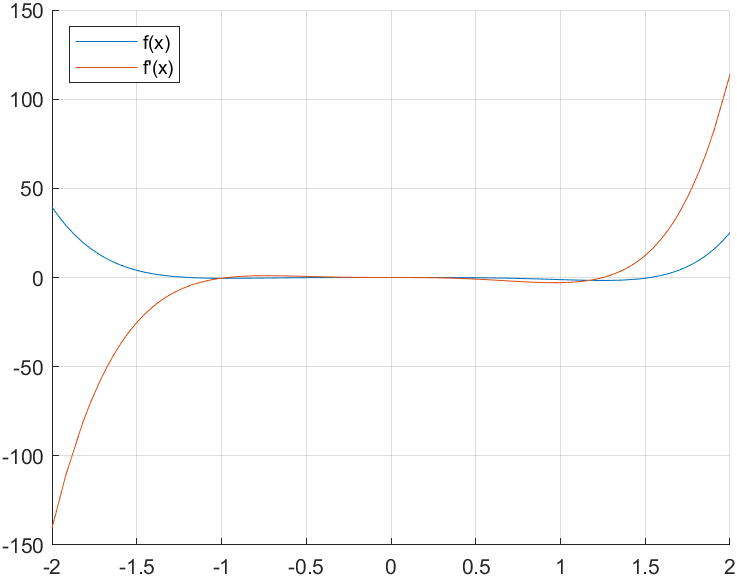
\includegraphics[width=\textwidth]{exercise1plot.png}
\end{figure}

Από το γράφημα παρατηρούμε ότι:
\begin{enumerate}
    \item Η f φαίνεται να έχει ρίζες κοντά στα $x_1=-1$, $x_2=0$ και $x_3=1.5$.
    \item Η f' έχει ρίζα στο 0.
\end{enumerate}
% Με το πρόγραμμα exercise_1.m υπολογίζουμε τις 
% \begin{center}
%     \emph{{\tiny Α}{\scriptsize Β}{\footnotesize Γ}{\small Δ}{\normalsize Ε}{\large Ζ}{\Large Η}{\LARGE Θ}{\Huge Ι}{\huge κ}{\LARGE λ}{\Large μ}{\large ν}{\normalsize ξ}{\small ο}{\footnotesize π}{\scriptsize ρ}{\tiny σ}}   
% \end{center}

% \section{Δεύτερη Άσκηση}
% \begin{center}
%     {\textit{Normal Italics \textbf{Bold}\\ \emph{E}mphasized \underline{Underlined}}} 
% \end{center}
% \pagebreak

% \section{Τρίτη Άσκηση}
% \begin{center}
%     {\large
%         $$a^2 + b^2 = c^2$$
%         $$e^{i\pi}=-1$$
%         $$\pi = \frac{c}{d}$$
%         $$\frac{d}{dx}\int_a^xf(s)ds = f(x)$$
%         $$f(x) = \sum_{\substack{i=0}}^{\substack{\infty}}\frac{f^{(i)}(0)}{i!}x^i$$
%         \textbf{Ax = b}
%         $$\|(x+y)\| \le \|x\|+\|y\|$$
%         \newline
%         \begin{equation}
%             I = \begin{pmatrix}
%                 1 & 0 & 0 & 0 \\
%                 0 & 1 & 0 & 0 \\
%                 0 & 0 & 1 & 0 \\
%                 0 & 0 & 0 & 1
%             \end{pmatrix}
%         \end{equation}
%         \newline
%         \begin{equation}
%             I = \begin{bmatrix}
%                 1 & 0 & 0 & 0 \\
%                 0 & 1 & 0 & 0 \\
%                 0 & 0 & 1 & 0 \\
%             0 & 0 & 0 & 1
%         \end{bmatrix}
%     \end{equation}
%     \newline
%     \begin{equation}
%         I = \begin{Bmatrix}
%             1 & 0 & 0 & 0 \\
%             0 & 1 & 0 & 0 \\
%             0 & 0 & 1 & 0 \\
%             0 & 0 & 0 & 1
%         \end{Bmatrix},\quad
%         I = \begin{vmatrix}
%             1 & 0 & 0 & 0 \\
%             0 & 1 & 0 & 0 \\
%             0 & 0 & 1 & 0 \\
%             0 & 0 & 0 & 1
%         \end{vmatrix},\quad
%         I = \begin{Vmatrix}
%             1 & 0 & 0 & 0 \\
%             0 & 1 & 0 & 0 \\
%             0 & 0 & 1 & 0 \\
%             0 & 0 & 0 & 1
%         \end{Vmatrix}                   
%     \end{equation}
%     }
% \end{center}
% \pagebreak

% \section{Τέταρτη Άσκηση}
% \begin{center}
%     {\itshape
%     \begin{tabular}{ c c c}
%         Τέφας & 2 & 3 \\
%         Πήτας & 5 & 6 \\
%         Λάσκαρης & 8 & 9 
%     \end{tabular}
    
%     \vspace{8mm}
%     \begin{tabular}{|c|c|c|}
%         Κοτρόπουλος & 6 & 3\\
%         Πήτας & 5 & 6 \\
%         Νικολαίδης & 8 & 9
%     \end{tabular}
    
%     \vspace{8mm}
%     \begin{tabular}{|c|c|c|}
%         \hline
%         1 & 2 & 3 \\
%         \hline
%         4 & 5 & 6 \\
%         \hline
%         7 & 8 & 9 \\
%         \hline
%     \end{tabular}
    
%     \vspace{8mm}
%     \begin{tabular}{|c|c|c|}
%         \hline
%         1 & 2 & 3 \\
%             \hline
%             4 & 5 & 6 \\
%             \hline
%             7 & 8 & 9 \\
%             \hline
%         \end{tabular}
    
%         \vspace{8mm}
%         \begin{tabular}{|c|c|l|}
%             \hline
%             \multicolumn{3}{|c|}{Μέλη ΔΕΠ Πληροφορικής}\\
%             \hline
%             Λέκτορες & VD & Δραζιώτης Κωνσταντίνος \\
%             \hline
%             \multirow{2}{6em}{Επίκουροι} & LN & Λάσκαρης Νικόλαος \\ 
%                 & TG  & Τσουμάκας Γρηγόριος \\
%             \hline
%             \multirow{3}{6em}{Αναπληρωτές} & TA & Τέφας Αναστάσιος \\
%                 & PN & Πλέρος Νίκος \\
%                 & PA & Παπαδόπουλος Απόστολος\\
%             \hline
%             \multirow{3}{6em}{Καθηγητές} & KC & Κοτρόπουλος Κωνσταντίνος \\
%                 & PI & Πήτας Ιωάννης \\
%                 & VI & Βλαχάβας Ιωάννης \\
%             \hline
%         \end{tabular}
%     }    
% \end{center}

% \section{Πέμπτη Άσκηση}
% \begin{itemize}
%     \item Τέφας
%     \item Μπουζάς
%     \item Μπρούζα
%     \item Λάσκαρης
%     \item Κοτρόπουλος
%     \item Πήτας
%     \item Νικολαΐδης
% \end{itemize}

\end{document}